\documentclass[tikz,border=5mm]{standalone}
\usepackage{pgfplots}
\usepackage{pgfplotstable}
\pgfplotsset{compat=1.17}

\begin{document}
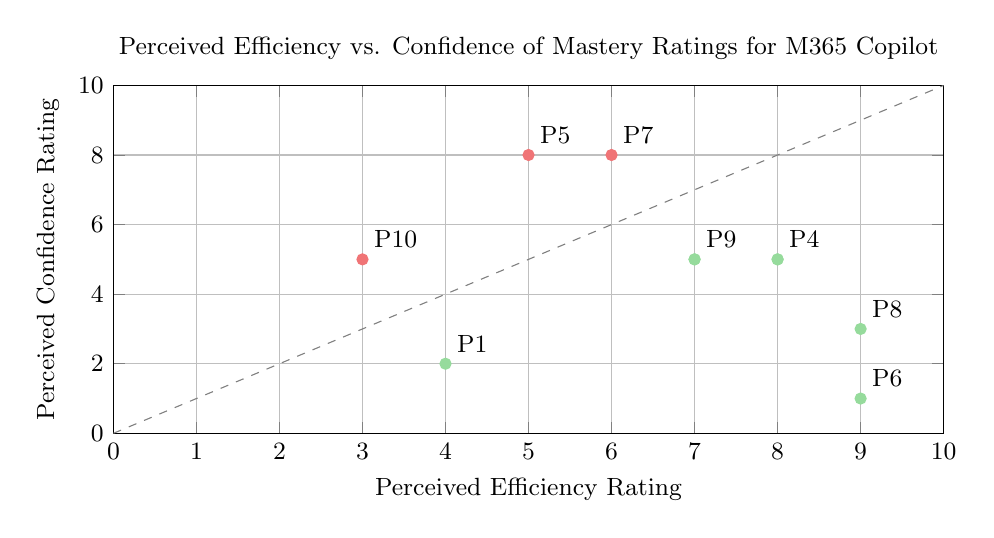
\begin{tikzpicture}
\definecolor{red}{RGB}{240,116,118}
\definecolor{green}{RGB}{150,219,156}
  \begin{axis}[
      xlabel={Perceived Efficiency Rating},
      ylabel={Perceived Confidence Rating},
      xmin=0, xmax=10,
      ymin=0, ymax=10,
      grid=both,
      width=\linewidth,           % Fit within a single column
      height=6cm,                 % Adjust height as needed
      title={Perceived Efficiency vs. Confidence of Mastery Ratings for M365 Copilot},
      title style={font=\small},
      label style={font=\small},
      tick label style={font=\small},
  ]
    % Dashed reference line y = x
    \addplot [domain=0:10, dashed, color=gray] {x};
    
    % Points above the reference line (Confidence > Efficiency)
    \addplot+[only marks, mark=*, color = Black,
      point meta=explicit symbolic,
      nodes near coords={\pgfplotspointmeta},
      nodes near coords style={
         anchor=south west, 
         font=\small, 
         fill=white, 
         inner sep=1pt,
         xshift=3pt,
         yshift=3pt
      },
      mark options ={fill=red, draw=red}
    ] coordinates {
      (5,8)[P5]
      (6,8)[P7]
      (3,5)[P10]
    };
    
    % Points below (or on) the reference line (Confidence <= Efficiency)
    \addplot+[only marks, mark=*, color = black,
      point meta=explicit symbolic,
      nodes near coords={\pgfplotspointmeta},
      nodes near coords style={
         anchor=south west, 
         font=\small, 
         fill=white, 
         inner sep=1pt,
         xshift=3pt,
         yshift=3pt
      },
       mark options ={fill=green, draw=green}
    ] coordinates {
      (4,2)[P1]
      (7,5)[P2]
      (8,5)[P3]
      (8,5)[P4]
      (9,1)[P6]
      (9,3)[P8]
      (7,5)[P9]
    };
    
\end{axis}
\end{tikzpicture}

\end{document}
